% \documentclass[dvipdfmx,autodetect-engine, 12pt]{jsarticle}

% \usepackage{ulem} % 取消線を引くためのパッケージ
% \usepackage[dvipdfmx]{graphicx} % 画像を挿入するためのパッケージ
% \usepackage{array} % 表の幅指定や自動改行に必要
% \usepackage{enumitem}

% % --- 考文献用の設定 ---
% \usepackage[backend=biber, style=numeric]{biblatex} % biblatexパッケージの使用
% \addbibresource{../source.bib} % 先ほど作った別ファイルを指定（拡張子まで書く）
% \usepackage{url} % WebサイトのURLを綺麗に出力するため

% % --- section の文字サイズを小さくする設定 ---
% \makeatletter
% \renewcommand{\section}{%
%   \@startsection{section}{1}{\z@}%
%   {1.5ex \@plus .5ex \@minus .2ex}% 前の行との隙間
%   {0.5ex \@plus .3ex}% 下の行との隙間
%   {\normalfont\normalsize}% ← ここでサイズを \Large（少し大きめ）に指定
% }
% \makeatother

% \begin{document}

% 課題のタイトル
\begin{center}

{\LARGE \bfseries 課題⑤\, iptablesによるポート転送\par}

\end{center}

\vspace{1cm}

{\LARGE \uline{目的}} \\

\hangindent=1.5zw
\hangafter=0
\noindent
iptables を用いたパケットの制御の実習を行う. パケットを分析することによりポート
転送の方法を確認する．

\vspace{1cm}

{\LARGE \uline{事前準備}} 

\begin{enumerate}
    \item server と router の VM を起動する．
    \item iptables コマンドについて調査する.
\end{enumerate}

\vspace{1cm}

{\LARGE \uline{手順}} 

\begin{enumerate}

    \item router で dropbear が起動していないことを確認し，起動している場合は停止する．
    
        \vspace{\baselineskip}
        \quad
        図\ref{fig:no_dropbear} は router で dropbear が起動していないことを確認する様子である．

        \begin{figure}[htbp]
            \centering
            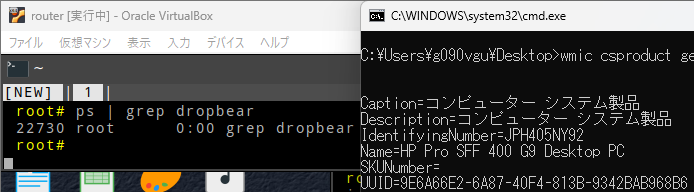
\includegraphics[width=0.8\textwidth]{imgs/no_dropbear.png} 
            \caption{server で dropbear が起動していないことの確認}
            \label{fig:no_dropbear}
        \end{figure}

        \quad
        ps コマンドで プロセス一覧を取得し, その結果をgrep コマンドでdropbearという文字列を含むものに限定している.
        フィルタリングされたプロセス一覧には, grep dropbear(プロセス一覧からの文字列検索に用いたコマンド)以外のコマンドによるプロセスは表示されていない.
        したがって, routerにおいてdropbearが起動していないことが確認できる.

        \vspace{\baselineskip}

    \item server で dropbear を -R オプション付きで起動し，起動を確認する．\\

        \quad
        図\ref{fig:dropbear_active}は server で dropbear を -R オプション付きで起動し，起動を確認する様子である.

        \begin{figure}[htbp]
            \centering
            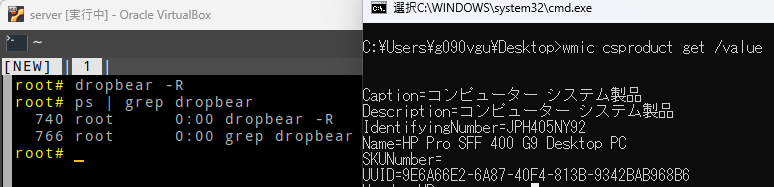
\includegraphics[width=0.8\textwidth]{imgs/server_dropbear_active.png} 
            \caption{server で dropbear 起動確認}
            \label{fig:dropbear_active}
        \end{figure}

        \quad
        ここではプロセス一覧において dropbear -R というコマンドで起動されたプロセスが表示されていることから, 
        dropbearが-Rオプション付きで起動していることが確認できる.\\

    \item デスクトップ PC(Windows) から router へ ssh で一般権限ユーザでログインできないことを確認する．
    
        \vspace{\baselineskip}
        \quad
        図\ref{fig:ssh_failed} はデスクトップPCからrouterへのssh接続に失敗する様子である.
    
        \begin{figure}[htbp]
            \centering
            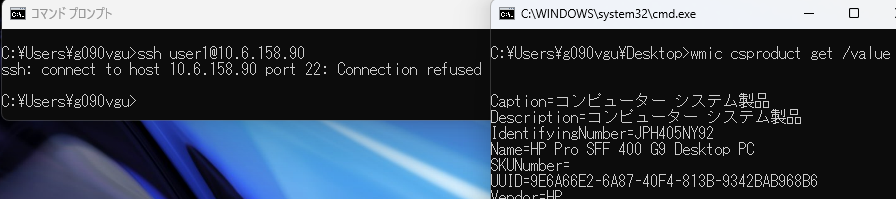
\includegraphics[width=0.8\textwidth]{imgs/ssh_failed.png} 
            \caption{デスクトップPCからrouterへのssh接続に失敗する様子}
            \label{fig:ssh_failed}
        \end{figure}

        \quad
        ssh: connect to host 10.6.158.90 port 22: Connection refused というエラーメッセージが表示されている.
        手順1で確認したとおり, routerにおいてはdropbearのプロセスが起動されていないためである.\\

    \item router の組織外側インターフェースに対して以下の iptables 設定を行う（必要なら sysctl で転送を有効化：net.ipv4.ip\_forward=1）：
    
    \begin{enumerate}[label=\textcircled{\scriptsize\arabic*}]
        \item TCP 22 番ポート宛てのパケットを server の TCP 22 番ポートへ転送する（例：PREROUTING で DNAT を設定）。
        \item TCP のそれ以外のポート宛てアクセスは転送しない（DROP/REJECT を設定）。
    \end{enumerate}

        \vspace{\baselineskip}
        \quad
        図\ref{fig:set_iptables_4}は手順4の要件を満たすようなiptablesの設定を行うコマンドの実行結果である.

        \begin{figure}[htbp]
            \centering
            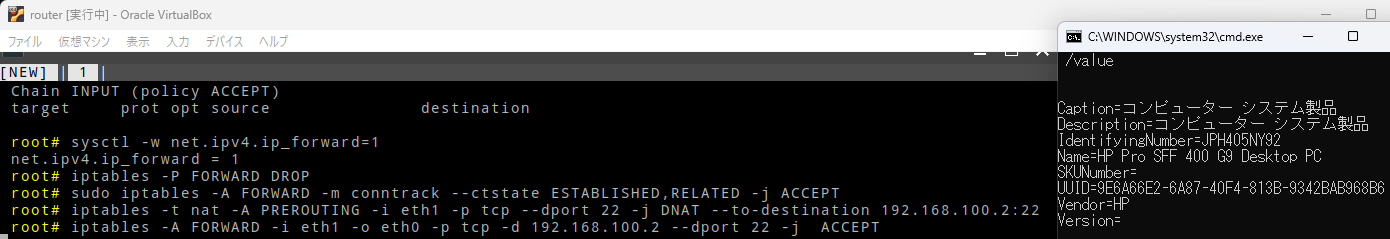
\includegraphics[width=0.8\textwidth]{imgs/set_iptables_4.png} 
            \caption{手順4の要件を満たすためのiptablesの編集コマンド}
            \label{fig:set_iptables_4}
        \end{figure}

        \quad
        ここで行った設定についてコマンドごとに説明を行う。\\

        \texttt{\# sysctl -w net.ipv4.ip\_forward=1} \\

        \texttt{sysctl}コマンド\cite{kazmax_sysctl_2022}を\texttt{-w}オプションで用いて，\texttt{net.ipv4.ip\_forward}の値を1に設定することで，ポートフォワーディングを有効化した。\\

        \texttt{\# iptables -P FORWARD DROP} \\

        明示的に許可した通信以外は転送しないようにするため，
        \texttt{-P}オプションによって対象のチェインのポリシーを設定している．
        ここでは\texttt{filter}テーブル上の\texttt{FORWARD}チェインに対して\texttt{DROP}というポリシーを設定し，
        デフォルトですべてのパケットを転送できないよう設定している\cite{man:iptables}．\\

        \texttt{\# iptables -A FORWARD -m conntrack --ctstate ESTABLISHED,RELATED -j ACCEPT} \\
        
        iptablesにおける接続追跡機能である\texttt{conntrack}の\texttt{--ctstate}オプションで\texttt{ESTABLISHED}と\texttt{RELATED}のステートリストを指定して，
        それらに該当するパケットの通信を許可することによって\cite{man_iptables_extensions_8}，
        既に確立済み（ESTABLISHED）または関連する（RELATED）通信のパケットを許可し，応答パケットを転送できるようにした.
        これによってserverからwindowsへの応答パケットの転送が可能となる.\\

        \texttt{\# iptables -t nat -A PREROUTING -i eth1 -p tcp --dport 22 -j DNAT --to-destination 192.168.100.2:22} \\
        
        \texttt{nat}テーブルの\texttt{PREROUTING}チェインに対して，\texttt{eth1}から自身に対して送信されたTCP 22番ポートへのパケットを，宛先IPアドレス「192.168.100.2」，宛先ポート「TCP 22番」へと書き換えるDNAT（宛先IPアドレスの書き換え）の設定を行っている．これにより\texttt{eth1}から自身の22番ポートへ送られたパケットは，サーバーの22番ポートに転送される．\\

        \texttt{\# iptables -A FORWARD -i eth1 -o eth0 -p tcp -d 192.168.100.2 --dport 22 -j ACCEPT} \\
        
        \texttt{filter}テーブルの\texttt{FORWARD}チェインに対して，\texttt{eth1}から送信された宛先IPアドレスが「192.168.100.2」で宛先ポートがTCP 22番のパケットの転送を許可する設定を行っている．これによって，DNATで宛先IPアドレスが変換されたパケットをサーバーの22番ポートに転送することが可能になる．\\


    \item Windows から router へ通信を発生させ，server に一般権限ユーザでログインできることを確認する（必要に応じて known\_hosts を編集して Host key 問題を解決する）．\\
    
        \quad
        図\ref{fig:ssh_login_success} はデスクトップPCからrouterへのssh接続を試みた結果である.

        \begin{figure}[htbp]
            \centering
            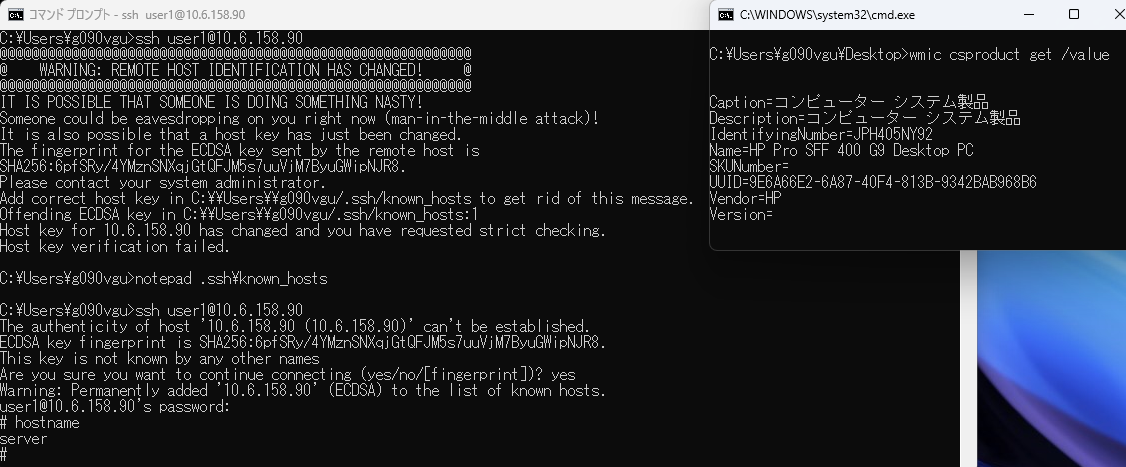
\includegraphics[width=0.8\textwidth]{imgs/ssh_win2sever_via_router.png} 
            \caption{デスクトップPCからrouterへのssh接続に成功する様子}
            \label{fig:ssh_login_success}
        \end{figure}

        \quad
        sshコマンドを実行すると, "remote host identification has changed!"
        と警告が発生していることがわかる.
        一般にsshのソフトウェアでは, $\sim$/.ssh/known\_hostsに接続先のサーバの公開鍵情報が保存される.
        次回接続した際には, ここに保存された公開鍵と照合することによって同じサーバかどうかを検証する\cite{zenn_known_hosts_2025},
        このときに公開鍵の情報が一致しなければ, 今回得られたような警告文が出力される.\\
        \quad
        今回の場合においては以前にwindowsからrouterに対してssh接続した際にrouterの公開鍵情報が$\sim$/.ssh/known\_hosts
        に保存されており, 今回も同じようにrouterに対してssh接続のコマンドを実行したが, 手順4においてsshのパケットを
        serverに転送するよう設定したことで, serverの公開鍵情報と以前に保存したrouterの公開鍵情報とで照合が行われ,
        一致せずに警告が発されたと考えられる. 
        ここでは記録されていたrouterの公開鍵情報を 
        $\sim$/.ssh/known\_hostsから削除することで対処した.
        結果として, 最終的にwindowsからserverにuser1としてログインできていることが確認できる.\\

    \item router 上で Wireshark を起動し，Windows↔router および router↔server の両方のインターフェースをキャプチャ対象に設定する．

    \item Windows から router への SSH ログイン過程のパケットを router の Wireshark で解析し，iptables による転送（IP アドレスやポート番号の書き換え）が観測できるパケットを特定する．
    
        \vspace{\baselineskip}
        \quad
        図\ref{fig:ssh_login_result}はrouter上でWiresharkを起動し, Windows↔router および router↔server の両方のインターフェースをキャプチャ対象に設定した様子である.
        % ここではキャプチャするパケットは, Windows↔router および router↔server を流れるパケットにに限定するため, wiresharkのフィルタに
        % (ip.src==192.168.100.1 and ip.dst==192.168.100.2) or (ip.src==192.168.100.2 and ip.dst==192.168.100.1)
        % と
        % (ip.src==10.6.158.90 and ip.dst==10.6.158.153) or (ip.src==10.6.158.153 and ip.dst==10.6.158.90)
        % を設定している.
        % 前述のようにフィルタリングした上で, 
        両方のインターフェースを流れるパケットを比較すると, プロトコルやパケット内の情報が類似していることが確認できる.
        実際に, １つパケットを抽出して比較した例を図\ref{fig:same_packet_example}に示す.

        \begin{figure}[htbp]
            \centering
            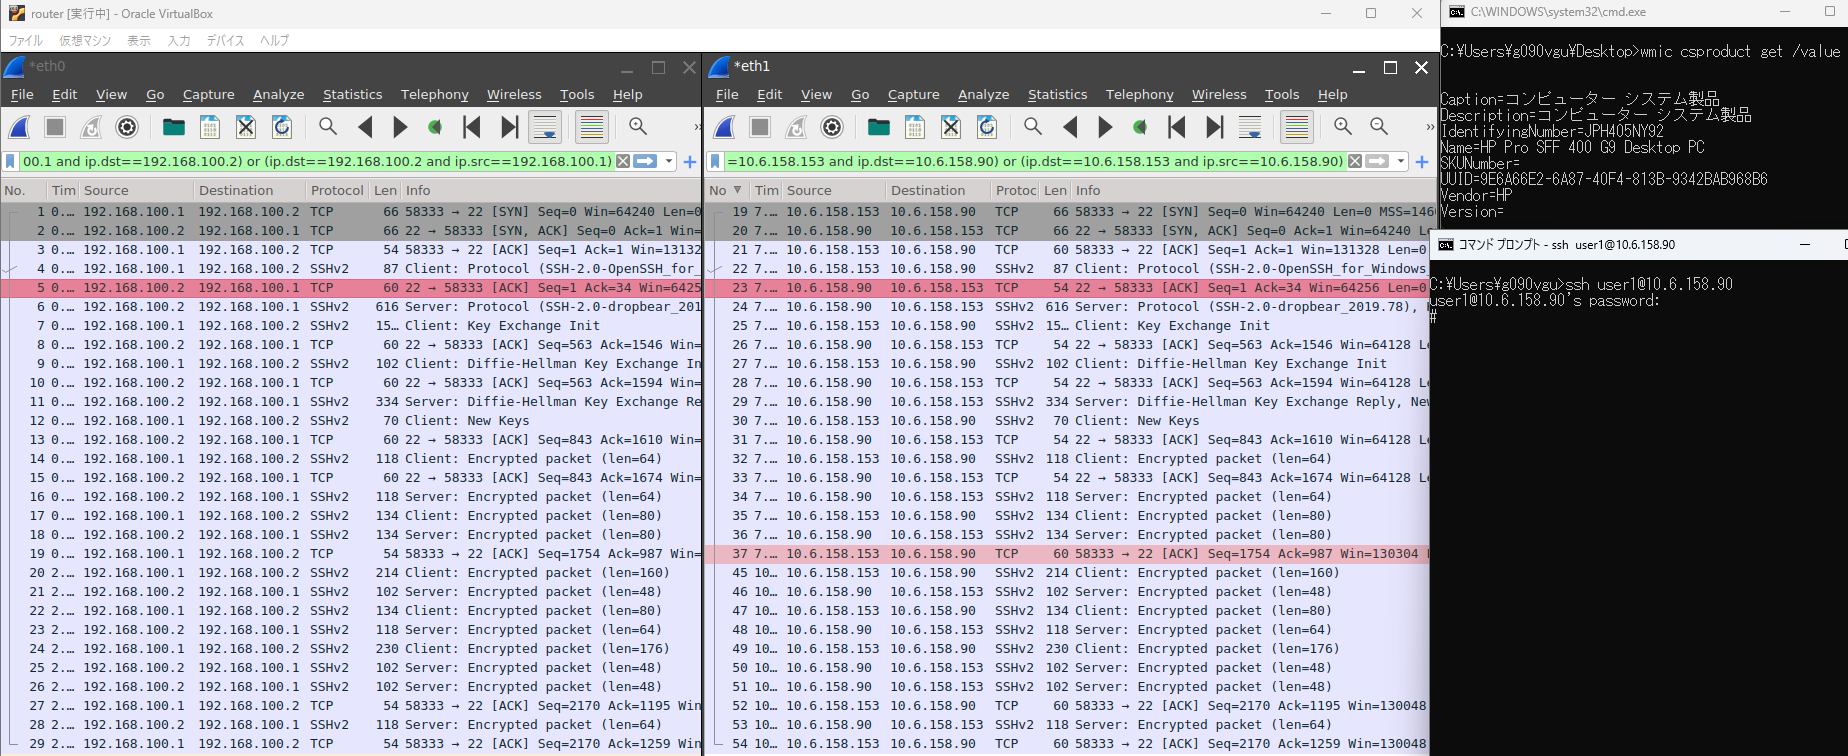
\includegraphics[width=0.8\textwidth]{imgs/ssh_login_result.png} 
            \caption{sshログイン時のWiresharkのキャプチャ結果}
            \label{fig:ssh_login_result}
        \end{figure}

        \begin{figure}[htbp]
            \centering
            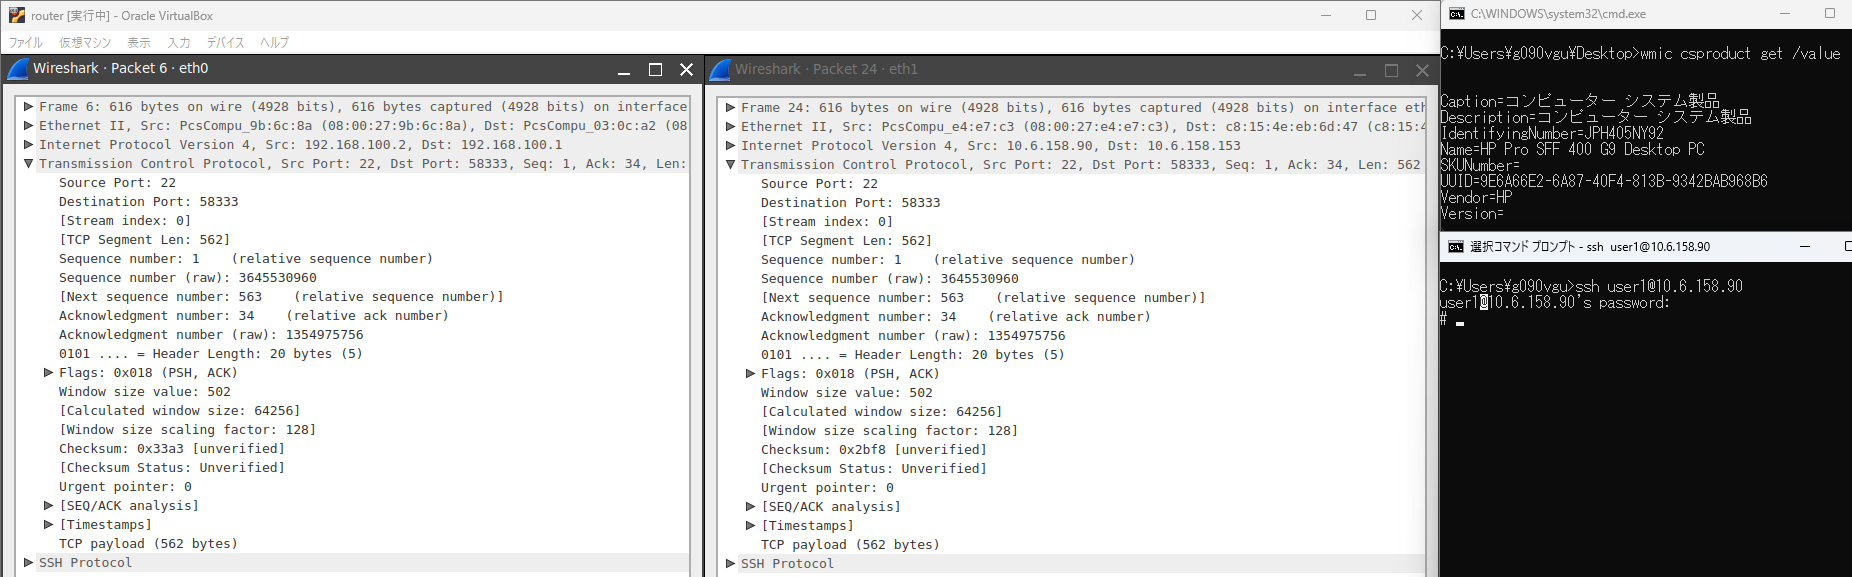
\includegraphics[width=0.8\textwidth]{imgs/same_packet_example.png} 
            \caption{Windows↔router および router↔server を流れるパケットの比較例}
            \label{fig:same_packet_example}
        \end{figure}

        \quad
        図\ref{fig:same_packet_example}に示すパケットは,それぞれrouterのeth0, eth1で観測されたSSHv2のパケットである.
        tcpのヘッダにおいて, フィールドの値(\texttt{Sequensce Number(raw): 3645530960, Acknowledgment Number(raw): 1354975756 など})が完全一致しており,
        転送されているものであるといえる.
        ここでは, server(192.168.100.2)のTCP 22番ポートからrouter(192.168.100.1)のTCP 58333番ポートへ送信されたパケットが, 
        router(10.6.158.90)のTCP 22番ポートからwindows(10.6.158.153)のTCP 58333番ポートへ送信されたパケットとして,
        宛先IPアドレス, 送信元IPアドレスがともに書き換えられていることが分かる.

        \vspace{\baselineskip}
    
    \item router の組織内側インターフェースに対して，server から組織外側ネットワークへの通信が可能になるように iptables を設定する（例：POSTROUTING で SNAT/MASQUERADE を設定）．
    
        \vspace{\baselineskip}

        図\ref{fig:set_iptables_7}は, 手順9の要件を満たすためのiptablesの編集コマンドの実行結果である.
        
        \begin{figure}[htbp]
            \centering
            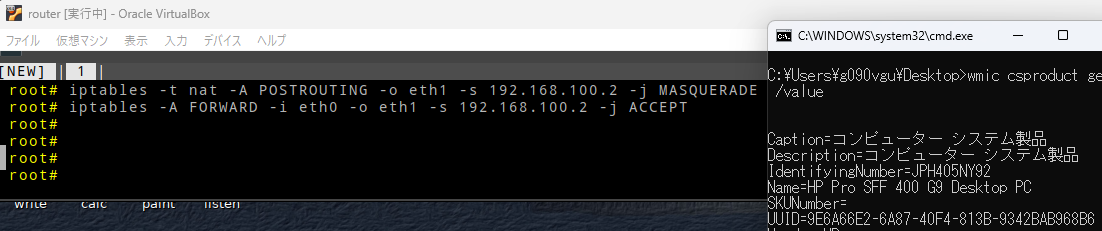
\includegraphics[width=0.8\textwidth]{imgs/set_iptables_8.png} 
            \caption{手順9の要件を満たすためのiptablesの編集コマンド}
            \label{fig:set_iptables_7}
        \end{figure}

        \quad
        ここで行った設定についてコマンドごとに説明を行う。\\

        \texttt{\# iptables -t nat -A POSTROUTING -o eth1 -s 192.168.100.2 -j MASQUERADE} \\

        \texttt{nat}テーブルの\texttt{POSTROUTING}チェインに対して，内部のサーバー（192.168.100.2）から\texttt{eth1}を経由して外部へ出ていく通信の送信元IPアドレスを，ルーターの外部IPアドレスへと書き換えるIPマスカレードの設定を行っている．\\

        \texttt{\# iptables -A FORWARD -i eth0 -o eth1 -s 192.168.100.2 -j ACCEPT} \\

        \texttt{filter}テーブルの\texttt{FORWARD}チェインに対して，\texttt{eth0}から受信して\texttt{eth1}から送信される，サーバー（192.168.100.2）から外部へ向かうパケットの転送を許可する設定を行っている．\\

        \vspace{\baselineskip}

    \item server から組織外ネットワークの端末へ通信を発生させ，router の Wireshark で解析し，iptables による変換（送信元 IP の書き換え等）を示すパケットを特定する．
    
        \vspace{\baselineskip}

        \quad
        図\ref{fig:server2windows_terminal}は, serverからwindowsに対してpingコマンドを実行した結果である.
        \begin{figure}[htbp]
            \centering
            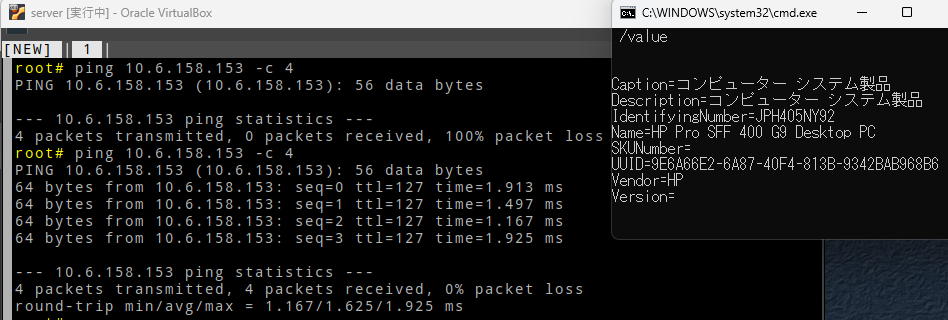
\includegraphics[width=0.8\textwidth]{imgs/ping_server2windows.png} 
            \caption{serverからwindowsに対するpingコマンドの実行結果}
            \label{fig:server2windows_terminal}
        \end{figure}

        \quad
        windowsからの応答が確認でき, serverとwindowsとの間で通信が可能であることが確認できる.\\
        \quad
        続いて, 図\ref{fig:masquerade_result}にserverからwindowsに対してpingコマンドを実行した際に
        キャプチャされたパケットの一覧を示す.

        \begin{figure}[htbp]
            \centering
            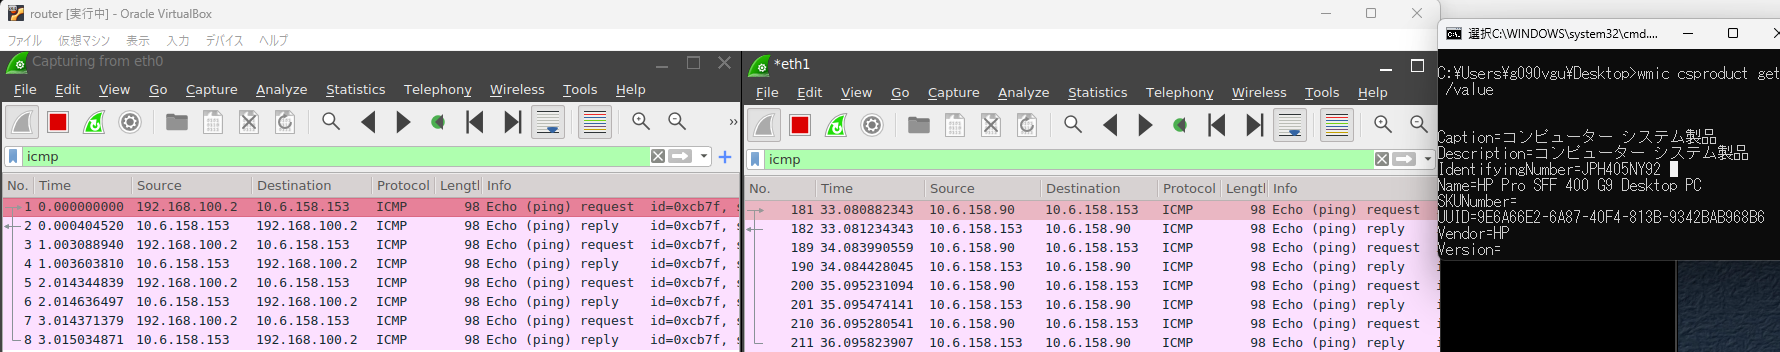
\includegraphics[width=0.8\textwidth]{imgs/prove_masquarade.png} 
            \caption{serverからwindowsに対するpingコマンド実行時にキャプチャされたパケット一覧}
            \label{fig:masquerade_result}
        \end{figure}      
        
        \quad
        左がeth0でのキャプチャ結果, 右がeth1でのキャプチャ結果である.
        ここで, eth0においてserver(192.168.100.2)からwindows(10.6.158.153)に対して送信されたICMPのパケットが,
        eth1においては, routerの外部アドレス(10.6.158.90)からwindows(10.6.158.153)に対してのパケットとして転送されていること,
        あるいはその逆のケースについても確認ができる.
        




        \vspace{\baselineskip}
    
    \item 実験結果として，デスクトップ PC から server へログインできること，
    server から組織外ネットワークへ通信できることを示し，
    使用したすべての iptables 設定を列挙する．
    各設定がどのようにパケットを書き換え，
    転送処理を実現しているかを具体的に説明してレポートにまとめる．\\

        \quad
        手順5,\, 9においてそれぞれ転送によってデスクトップPCからserverにログインできることと
        組織外ネットワークに属する装置と通信ができることが確認できた.\\
        \quad
        また, 手順7,\, 9においてパケットのiptablesによる転送処理(パケットの書き換え)が実現されていることが確認できた.\\
        \quad
        ここでは各通信の実現に必要な設定についても各手順で述べたとおりであるが,
        serverから組織外ネットワークへの通信に必要な設定について,
        デスクトップPCからserverにログインできるために必要な設定と重複して,
        手順9で述べられていない部分があるため,
        ここではその点に対する補足を行う.\\
        \quad
        まずはカーネルパラメータの設定で, 
        コマンドにすると以下のとおりである.\\

        \texttt{\# sysctl -w net.ipv4.ip\_forward=1} \\

        の部分で, 
        これは2つのNIC間でのパケットの転送を許可するためのパラメータを設定するものであり,
        ルータとして機能させるためには必須の設定のためである.
        この実験ネットワークでは, 
        具体的にrouterのeth1から届いたパケットをeth0から転送したい際,あるいはその逆の場合に
        ホスト(router)内インターフェース間でのパケットの転送を実現するものである.
        \\
        \quad
        もう一点が, iptablesの設定で,
        コマンドにすると以下のものである.\\

        \texttt{\# iptables -A FORWARD -m conntrack --ctstate ESTABLISHED,RELATED -j ACCEPT} \\

        これは, 一度通信が確立された後の帰りのパケットを転送するための設定である.\\
        手順9では, 組織内から組織外へパケットを送信する際に, routerの組織外とのインターフェースを用いて通信を行うための設定は行っているが,
        応答パケットを転送するための設定は行っていない. 
        したがって, ここでこの設定を行うことによって, 双方向の通信が実現される.
        

        \quad
        
        
        

\end{enumerate}

\newpage

% % --- 参考文献リストの出力 ---
% \printbibliography[title=参考文献]

% \end{document}